\chapter{Planning}
In dit hoofdstuk wordt de initiële planning beschreven, en daarbij de verschillende deadlines voor de op te leveren producten.
Verder wordt er een strokenplanning beschreven in hoofdstuk \ref{sec:strokenplanning}.
\section{Op te leveren producten}
De deadlines en concept versies van de verschillende eindproducten worden beschreven in Tabel \ref{tab:Deadline}.

\whitespace[2]
\begin{graphic}
	\captionsetup{type=table}
	\begin{tabularx}{\textwidth}{|l|l|X|}
		\hline
		\textbf{Op te leveren producten} & \textbf{Conceptversie} & \textbf{Deadline}        \\
		\hline
		Plan van aanpak                  & 5-10-2023              & 13-10-2023               \\
		\hline
		Onderzoeksverslag                & 8-11-2023              & 22-11-2023               \\
		\hline
		Onderzoeksverslag (2de kans)     & 26-3-2023              & 12-4-2024                 \\
		\hline
		Technische verslag               & 26-3-2023              & 12-4-2024                 \\
		\hline
		Product                          & niet van toepassing    & 12-4-2024                 \\
		\hline
		Presentatie                      & 29-4-2024              & 6/7/8 mei 2024 \\
		\hline
	\end{tabularx}
	\caption{Deadlines en conceptversie inlever momenten}
	\label{tab:Deadline}
	\vspace{0.2cm}
\end{graphic}
\section{Strokenplanning}
\label{sec:strokenplanning}
In Figuur \ref{fig:StrokenPlanning} wordt de strokenplanning weergegeven, die een verwachting geeft van de verwachte voortgang van het project.
Deze planning omvat alle projectactiviteiten een vergrote versie is te vinden in bijlage \ref{appendix:Strokenplanning}.

\whitespace[2]
\begin{graphic}
	\captionsetup{type=figure}
	\caption{Voorlopige Strokenplanning}
	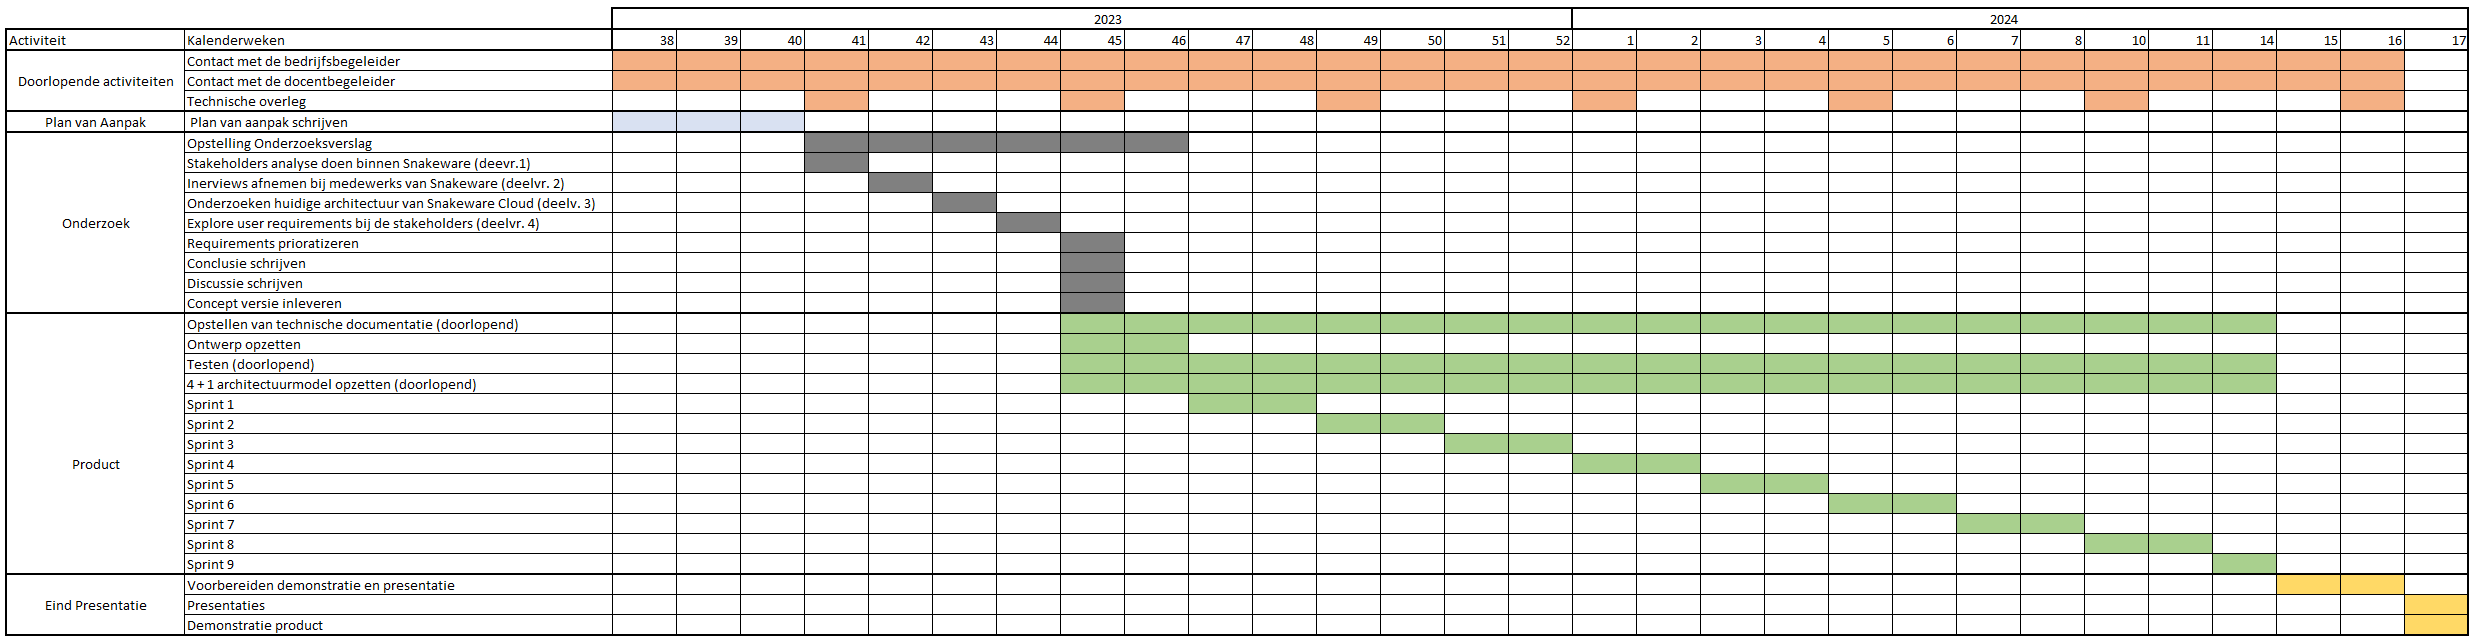
\includegraphics[scale=0.25]{StrokenPlanning}
	\label{fig:StrokenPlanning}
\end{graphic}
